\documentclass[fleqn, a4paper, 12pt]{article}
\usepackage{amsmath, amssymb, amsthm}
\usepackage{gensymb}
\usepackage{commath}
\usepackage{xcolor}
\usepackage{cancel}
\usepackage{siunitx}
\usepackage{tikz, pgfplots}
	\usetikzlibrary{calc, hobby, patterns, intersections}
\usepackage{graphicx}
\usepackage{hyperref}
\usepackage{datetime}
\usepackage{ulem}
\usepackage{xfrac}
\usepackage{asymptote}
\usepackage{enumerate}
\setcounter{secnumdepth}{4}
\newcommand\numberthis{\addtocounter{equation}{1}\tag{\theequation}}

\newcommand{\AxisRotator}[1][rotate=0]{%
	\tikz [x=0.25cm,y=0.60cm,line width=.2ex,-stealth,#1] \draw (0,0) arc (-150:150:1 and 1);%
}

\theoremstyle{definition}
\newtheorem{example}{Example}
\newtheorem{definition}{Definition}

\theoremstyle{theorem}
\newtheorem{theorem}{Theorem}

\newenvironment{solution}
{\begin{proof}[Solution]\let\qed\relax}
	{\end{proof}}

\newcommand{\curl}{\mathrm{curl\,}}

%\renewcommand{\int_{min}^{max}}{\int\displaylimits_{min}^{max}}

%opening
\title{Lecture 16}
\author{Aakash Jog}
\date{\formatdate{23}{12}{2014}}

\begin{document}

\maketitle
%\setlength{\mathindent}{0pt}

\tableofcontents

\newpage
\section{Rigid Body Collisions}

\subsection{Conservation of Angular Momentum}

If
\begin{equation*}
	\sum \overrightarrow{F_{\text{ext}}} = 0
\end{equation*}
then
\begin{align*}
	\overrightarrow{\tau_A} &= \sum \overrightarrow{r} \times \overrightarrow{F_{\text{ext}}}\\
	&= 0\\
	\therefore \dod{}{t}\overrightarrow{L_A} &= 0\\
	\therefore \overrightarrow{L_A} &= \text{ constant }
\end{align*}

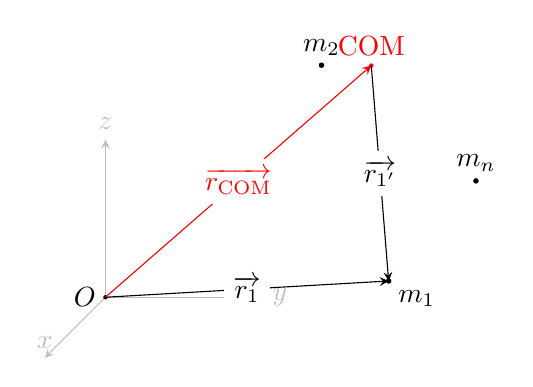
\begin{tikzpicture}
	%definition of origin
	\coordinate (O) at (0,0,0); 
	
	%definition of minimum and maximum values for axes
	\def\xMIN{0};
	\def\yMIN{0};
	\def\zMIN{0};
	\def\xMAX{2};
	\def\yMAX{2};
	\def\zMAX{2};
	
	%axes
	\draw [-stealth, lightgray] (\xMIN,0,0) -- (\xMAX,0,0) node [right] {$y$}; 
	\draw [-stealth, lightgray] (0,\yMIN,0) -- (0,\yMAX,0) node [above] {$z$};
	\draw [-stealth, lightgray] (0,0,\zMIN) -- (0,0,\zMAX) node [above] {$x$};
	
	\fill (O) circle [radius = 0.8pt] node [left] {$O$};
	
	%point masses
	\coordinate (m1) at (4+rnd, 1+rnd, 3+rnd);
	\coordinate (m2) at (2+rnd, 3+rnd, rnd);
	\coordinate (mn) at (5+rnd, 2+rnd, 2+rnd);
	
	\fill (m1) circle [radius = 1pt] node [below right] {$m_1$};
	\fill (m2) circle [radius = 1pt] node [above] {$m_2$};
	\fill (mn) circle [radius = 1pt] node [above] {$m_n$};
	
	%distances from origin
	\draw [-stealth] (O) -- (m1) node [midway, fill = white] {$\overrightarrow{r_1}$};
	
	%centre of mass
	\coordinate (COM) at (5+rnd, 5+rnd, 5+rnd);
	
	\fill [red] (COM) circle [radius = 0.8pt] node [above] {COM};
	
	\draw [-stealth, red] (O) -- (COM) node [midway, fill = white] {$\overrightarrow{r_\text{COM}}$};
	
	%distances from COM
	\draw [-stealth] (COM) -- (m1) node [midway, fill = white] {$\overrightarrow{r_{1'}}$};
\end{tikzpicture}

\begin{align*}
	\overrightarrow{L_O} &= \sum \overrightarrow{r_i} \times \left( m_i \overrightarrow{v_i} \right)\\
	&= \sum \left( \overrightarrow{r'_i} + \overrightarrow{r_{\text{COM}}} \right) \times \left(m_i \left(\overrightarrow{v_{\text{COM}}} + \overrightarrow{v'_i}\right)\right)\\
	&= \sum \overrightarrow{r'_i} \times \left(m_i \overrightarrow{v_{\text{COM}}}\right) + \sum \overrightarrow{r'_i} \times \left(m_i \overrightarrow{v'_i}\right) \\
	&\quad+ \sum \overrightarrow{r_\text{COM}} \times \left(m_i \overrightarrow{v_{\text{COM}}}\right) + \sum \overrightarrow{r_\text{COM}} \times \left(m_i \overrightarrow{v'_i}\right)\\
	&= \sum \cancelto{0}{\left(m_i \overrightarrow{r'_i}\right)} \times \overrightarrow{v_{\text{COM}}} + \overrightarrow{L_{COM}}\\
	&\quad + \overrightarrow{r_{\text{COM}}} \times \left( \sum m_i \right) \overrightarrow{v_{\text{COM}}} + \overrightarrow{r_{\text{COM}}} \cancelto{0}{\sum m_i \overrightarrow{v'_i}}\\
	&= \overrightarrow{L_{\text{COM}}} + \overrightarrow{r_{\text{COM}}} \times \left( \sum m_i \right) \overrightarrow{v_{\text{COM}}}
\end{align*}

\begin{example}
	Consider a system of two point masses rotating about their centre of mass, with $\omega_0$. Another point mass is positioned as shown. The masses collide and move with $\omega_1$. Find $\omega_1$.\\
	\begin{tikzpicture}
		%definition of origin
		\coordinate (O) at (0,0,0); 
		
		%variables
		\def\a{5};
		\def\angle{30};
		
		%point masses
		\coordinate (m1) at (\angle:\a);
		\coordinate (m2) at (180+\angle:\a);
		\coordinate (m3) at (-90:\a);
		
		\draw [dashed, green] (90:\a) -- (-90:\a);
		
		\fill (m1) circle [radius = 3pt] node [below right] {$m$};
		\fill (m2) circle [radius = 3pt] node [above] {$m$};
		\fill (m3) circle [radius = 3pt] node [above] {$m$};
		
		%centre of mass
		\coordinate (COM) at (-90:\a/3);
		
		\fill [green] (COM) circle [radius = 3pt] node [below right] {COM};
		
		%rod
		\draw (m1) -- (m2);
		
		%movement
		\draw [-stealth, red] (1,0) arc (0:300:1) node [right] {$\omega_0$};
		
		%dimensions
		\draw [|<->|] ($ (O) + (90+\angle:2) $) -- ($ (m1) + (90+\angle:2) $) node [midway, fill=white] {$a$};
		\draw [|<->|] ($ (O) + (90+\angle:2) $) -- ($ (m2) + (90+\angle:2) $) node [midway, fill=white] {$a$};
	\end{tikzpicture}
\end{example}

\begin{solution}
	Before the collision, wrt the COM of all 3 bodies,
	\begin{align*}
		\overrightarrow{L_{\text{COM}}} &= 0 + \dfrac{4a}{3} m a \omega_0 \hat{z} + \dfrac{2a}{3} m a \omega_0 \hat{z}\\
		&= 2 a^2 m \omega_0 \hat{z}
	\end{align*}
	After the collision, wrt the COM of all 3 bodies,
	\begin{align*}
		\dfrac{4}{3} a m \dfrac{4}{3} a \omega_1 \hat{z} + \dfrac{2}{3} a (2m) \dfrac{2}{3} a \omega_1 \hat{z}
	\end{align*}
	Applying COAM,
	\begin{align*}
		\omega_1 &= \dfrac{3}{4} \omega_0
	\end{align*}
\end{solution}

\begin{example}
	A particle of mass $m$ hits a system of 2 masses, as shown.\\
	\begin{tikzpicture}
		%definition of origin
		\coordinate (O) at (0,0,0); 
		
		%variables
		\def\a{5};
		\def\angle{90};
		
		%point masses
		\coordinate (m1) at (\angle:\a);
		\coordinate (m2) at (180+\angle:\a);
		\coordinate (m3) at (-\a, -5);
		
		\draw [dashed, green] (90:\a) -- (-90:\a);
		
		\fill (m1) circle [radius = 3pt] node [below right] {$m$};
		\fill (m2) circle [radius = 3pt] node [right] {$m$};
		\fill (m3) circle [radius = 3pt] node [above] {$m$};
		
		%centre of mass	
		\coordinate (A) at (-90:\a/3);
		
		\fill [red] (A) circle [radius = 2pt] node [below right] {A};
		
		%rod
		\draw (m1) -- (m2);
		
		%movement
		\draw [-stealth] (m3) -- ++(0:1) node [right] {$v_0$};
		
		%dimensions
		\draw [|<->|] ($ (O) + (90+\angle:-2) $) -- ($ (m1) + (90+\angle:-2) $) node [midway, fill=white] {$a$};
		\draw [|<->|] ($ (O) + (90+\angle:-2) $) -- ($ (m2) + (90+\angle:-2) $) node [midway, fill=white] {$a$};
		\draw [|<->|] ($ (A) + (90+\angle:-1) $) -- ($ (m2) + (90+\angle:-1) $) node [midway, fill=white] {$\dfrac{2}{3} a$};
	\end{tikzpicture}
\end{example}

\begin{solution}
	Before the collision,
	\begin{align*}
		\overrightarrow{L} &= \dfrac{2a}{3} m v_0 \hat{z}
	\end{align*}
	After the collision,
	\begin{align*}
		\overrightarrow{L} &= \overrightarrow{L'_{\text{COM}}} + \overrightarrow{r_{\text{COM}}} \times 3 m \dfrac{v_0}{3} \hat{x}\\
		&= \dfrac{4a}{3} m \dfrac{4a}{3} \omega \hat{z} + \dfrac{2a}{3} (2m) \dfrac{2a}{3} \omega \hat{z}
	\end{align*}
	Applying COAM,
	\begin{align*}
		\omega &= \dfrac{v_0}{4a}
	\end{align*}
\end{solution}

\begin{example}
	3 masses form an equilateral triangle of side length $L$. A particle of mass $m$ is moving towards the apex of the triangle as shown. Given that the particle moves with a velocity of $-\dfrac{v_0}{5} \hat{x}$ after the collision, and that the collision is inelastic, find \\
	\begin{tikzpicture}
		%definition of origin
		\coordinate (O) at (0,0,0); 
		
		%variables
		\def\l{5};
		
		%point masses
		\coordinate (m1) at (90:{\l/sqrt(3)});
		\coordinate (m2) at (210:{\l/sqrt(3)});
		\coordinate (m3) at (330:{\l/sqrt(3)});
		\coordinate (m4) at ({-2*\l/sqrt(3)}, {\l/sqrt(3)});
		
		\fill (m1) circle [radius = 3pt] node [above] {$m$};
		\fill (m2) circle [radius = 3pt] node [below] {$m$};
		\fill (m3) circle [radius = 3pt] node [below] {$m$};
		\fill (m4) circle [radius = 3pt] node [below] {$m$};
		
		%centre of mass	
	
		%triangle
		\draw (m1) -- (m2) -- (m3) -- cycle;
		
		%movement
		\draw [-stealth] (m4) -- ++(0:1) node [right] {$v_0$};

	\end{tikzpicture}
\end{example}

\begin{solution}
	Before the collision,
	\begin{align*}
		\overrightarrow{L_A} &= \dfrac{2}{3}L\dfrac{\sqrt{3}}{2} m v_0 (-\hat{z})
	\end{align*}
	After the collision,
	\begin{align*}
		\overrightarrow{L_A} &= \dfrac{2}{3} \cdot L \cdot \dfrac{\sqrt{3}}{2} \cdot m \dfrac{v_0}{5} \left( +\hat{z} \right) + \overrightarrow{L_{\triangle, A}}\\
		&= \dfrac{2}{3} \cdot L \dfrac{\sqrt{3}}{2} \cdot m \dfrac{v_0}{5} \left( +\hat{z} \right) + 3 d^2 m \omega \left( -\hat{z} \right) + \overrightarrow{r_{\text{COM}}} \times \left( 3m \cdot \dfrac{2}{5} \cdot v_0 \hat{x} \right)\\
		\therefore \omega &= \dfrac{2 \sqrt{3}}{5} \cdot \dfrac{v_0}{L}
	\end{align*}
\end{solution}

\section{Rigid Body Mechanics}

\begin{theorem}[Steiner Theorem (Theorem of Parallel Axes)]
	\begin{equation*}
		I = I_{\text{COM}} + M r^2_{\text{COM}}
	\end{equation*}
\end{theorem}

\begin{theorem}[Theorem of Perpendicular Axes]
	For a body in the $xy$-plane,
	\begin{equation*}
		I_z = I_x + I_y
	\end{equation*}
\end{theorem}

\end{document}